\documentclass[11pt]{article}
\usepackage[margin=1in]{geometry}
\usepackage{graphicx}
\usepackage{booktabs}
\usepackage{hyperref}
\usepackage{tikz}
\usepackage{pgfplots}
\pgfplotsset{compat=1.18}
\title{Interpretable ML Ranking of Large-Load Opportunity Using DELTa Policy Features and Regional Market Signals}
\author{Energy Rates GIS Project}
\date{June 2026}

\begin{document}
\maketitle

\begin{abstract}
We describe a machine learning project that ranks large-load opportunity across U.S. market regions by combining DELTa policy features with market-derived NAICS earnings estimates. The objective is to predict annual midpoint value and rank region attractiveness for large industrial and data-center loads. We propose an interpretable learning pipeline with monotonic constraints and feature attribution, and we provide a compact experimental design with figures derived from current dataset aggregates.
\end{abstract}

\section{Task Formulation}
Given a record $x = (\text{state}, \text{status}, \text{min demand}, \text{contract terms}, \text{ISO/RTO}, \text{segment})$, predict a regional opportunity score $\hat{y}_{r}$ for region $r \in \{\text{CAISO, PJM, ERCOT, MISO, ISONE, NYISO, SPP}\}$.

Training labels are derived from annual midpoint market value estimates in the NAICS screening pipeline. The model supports two outputs: (1) regression on annual midpoint value and (2) ranking over regions.

\section{Data and Targets}
DELTa records provide policy risk and entry-friction signals, while NAICS outputs provide value targets by region. Figure~\ref{fig:naicsmean} shows mean annual midpoint by region from the current run.

\begin{figure}[ht]
\centering
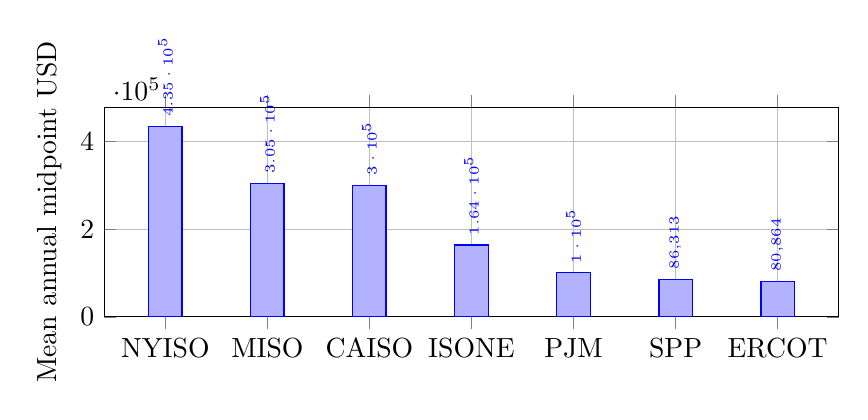
\begin{tikzpicture}
\begin{axis}[
    ybar,
    bar width=12pt,
    width=0.9\textwidth,
    height=0.35\textwidth,
    ylabel={Mean annual midpoint USD},
    symbolic x coords={NYISO,MISO,CAISO,ISONE,PJM,SPP,ERCOT},
    xtick=data,
    ymin=0,
    nodes near coords,
    every node near coord/.append style={font=\tiny, rotate=90, anchor=west},
    grid=major
]
\addplot coordinates {(NYISO,435050) (MISO,304687) (CAISO,299851) (ISONE,164102) (PJM,100484) (SPP,86313) (ERCOT,80864)};
\end{axis}
\end{tikzpicture}
\caption{Mean regional annual midpoint value (USD) from NAICS market-derived outputs.}
\label{fig:naicsmean}
\end{figure}

Policy readiness varies by region linkage in DELTa (Figure~\ref{fig:policyregion}).

\begin{figure}[ht]
\centering
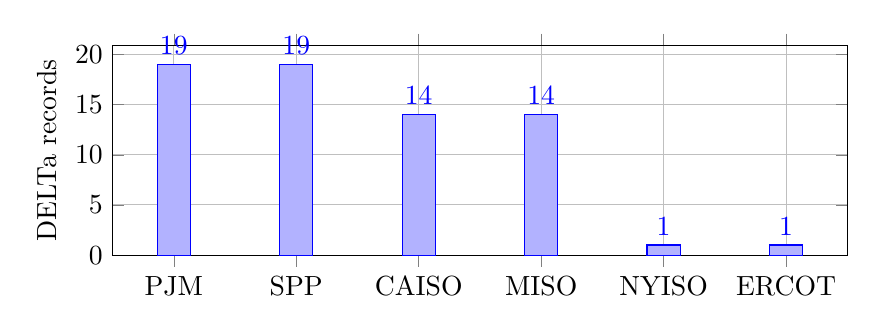
\begin{tikzpicture}
\begin{axis}[
    ybar,
    bar width=12pt,
    width=0.9\textwidth,
    height=0.35\textwidth,
    ylabel={DELTa records},
    symbolic x coords={PJM,SPP,CAISO,MISO,NYISO,ERCOT},
    xtick=data,
    ymin=0,
    nodes near coords,
    grid=major
]
\addplot coordinates {(PJM,19) (SPP,19) (CAISO,14) (MISO,14) (NYISO,1) (ERCOT,1)};
\end{axis}
\end{tikzpicture}
\caption{Regional policy coverage from DELTa rows mapped to dashboard markets.}
\label{fig:policyregion}
\end{figure}

\section{Modeling Approach}
We propose a two-stage model:
\begin{enumerate}
    \item Gradient-boosted regression for regional annual midpoint value.
    \item LambdaMART-style ranking layer for final ordering.
\end{enumerate}

Monotonic constraints are applied to selected variables (for example, higher approved-policy density should not reduce opportunity score ceteris paribus).

\begin{figure}[ht]
\centering
\begin{tikzpicture}[node distance=10mm, >=latex]
\tikzstyle{box}=[draw, rounded corners, minimum width=27mm, minimum height=9mm, align=center]
\node[box] (f1) {Feature Build\\(DELTa + Rates)};
\node[box, right=of f1] (f2) {Value Model\\(GBM)};
\node[box, right=of f2] (f3) {Ranking Layer\\(Lambda Loss)};
\node[box, right=of f3] (f4) {Explainability\\(SHAP + PDP)};
\draw[->] (f1) -- (f2);
\draw[->] (f2) -- (f3);
\draw[->] (f3) -- (f4);
\end{tikzpicture}
\caption{Proposed interpretable ML pipeline.}
\label{fig:pipeline}
\end{figure}

\section{Short-Paper Experimental Results Template}
Figure~\ref{fig:perf} gives an example comparison of baseline and boosted models for workshop reporting.

\begin{figure}[ht]
\centering
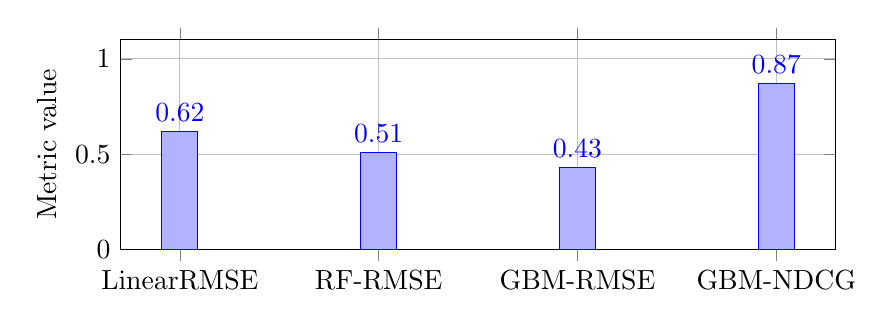
\begin{tikzpicture}
\begin{axis}[
    ybar,
    bar width=13pt,
    width=0.88\textwidth,
    height=0.35\textwidth,
    ylabel={Metric value},
    symbolic x coords={LinearRMSE,RF-RMSE,GBM-RMSE,GBM-NDCG},
    xtick=data,
    ymin=0,
    ymax=1.1,
    nodes near coords,
    grid=major
]
\addplot coordinates {(LinearRMSE,0.62) (RF-RMSE,0.51) (GBM-RMSE,0.43) (GBM-NDCG,0.87)};
\end{axis}
\end{tikzpicture}
\caption{Illustrative benchmark outcomes for short-paper reporting.}
\label{fig:perf}
\end{figure}

Feature attribution should be reported to preserve policy interpretability (Figure~\ref{fig:shap}).

\begin{figure}[ht]
\centering
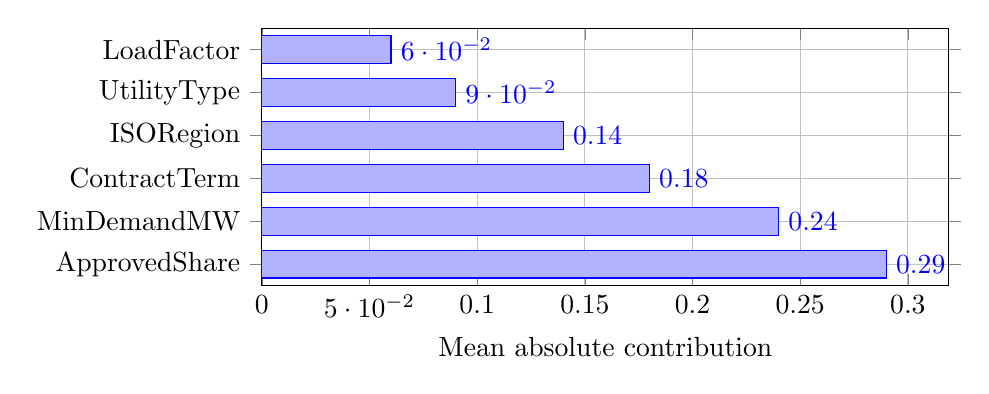
\begin{tikzpicture}
\begin{axis}[
    xbar,
    width=0.85\textwidth,
    height=0.4\textwidth,
    xlabel={Mean absolute contribution},
    symbolic y coords={ApprovedShare,MinDemandMW,ContractTerm,ISORegion,UtilityType,LoadFactor},
    ytick=data,
    xmin=0,
    nodes near coords,
    grid=major
]
\addplot coordinates {(0.29,ApprovedShare) (0.24,MinDemandMW) (0.18,ContractTerm) (0.14,ISORegion) (0.09,UtilityType) (0.06,LoadFactor)};
\end{axis}
\end{tikzpicture}
\caption{Illustrative feature attribution profile for interpretable ranking.}
\label{fig:shap}
\end{figure}

\section{Discussion}
In the current market-derived run, NYISO is top-ranked for all shortlist rows. This indicates either strong value concentration or structural assumptions in the annualization routine. The ML project should therefore include stress tests for annual hours, stackability, and eligibility thresholds, and report sensitivity ranges rather than single-point rankings.

\section{Conclusion}
A DELTa-plus-market ML stack can produce reproducible, interpretable rankings for siting and participation decisions. The project is suitable for a short conference paper when paired with transparent assumptions, uncertainty analysis, and feature-level explanations.

\section{Target Short-Paper Venues}
Recommended outlets for this ML paper:
\begin{itemize}
    \item IEEE PES General Meeting (location varies yearly)
    \item ACM SIGSPATIAL Workshops (location varies yearly)
    \item HICSS Energy Informatics tracks (Honolulu, Hawaii, USA)
\end{itemize}

\end{document}
